\documentclass{beamer}
\setbeamertemplate{bibliography item}{[\theenumiv]}

\usepackage[utf8]{inputenc}
\usepackage[normalem]{ulem}
\usepackage{url}
\usepackage{silence}
\usepackage[backend=bibtex]{biblatex}
\usepackage{etoolbox}
\usepackage{lipsum}
\usepackage{threeparttable}
\usetheme{Warsaw}
\bibliography{biblio}

\newcommand\Fontvi{\fontsize{6}{7.2}\selectfont}

% Reduce line spacing in table of contents
\makeatletter
\patchcmd{\beamer@sectionintoc}{\vskip1.5em}{\vskip0.5em}{}{}
\makeatother


% Reduce font size of footnotes
\renewcommand{\footnotesize}{\scriptsize}

% Ignore warnings regarding footnote
\WarningFilter{biblatex}{Patching footnotes failed}
\WarningFilter{biblatex}{Data encoding is 'utf8'}

\title{Authentication Mechanisms Using Raspberry Pi}
\author{
    Jon Kiefer S. Yap
    \and
    Matthew Kendrick D. Co}
\institute{University of the Philippines Diliman}

\begin{document}

\frame{\titlepage}

\AtBeginSection[] {
  \begin{frame}
  \small{
    \frametitle{Outline}
    \setcounter{tocdepth}{2}
    \tableofcontents[currentsection, hideothersubsections]
  }
  \end{frame}
}

\section{Introduction}
\subsection{Introduction}
\begin{frame}{Introduction}
\begin{itemize}
    \item<1-> The following are properties of modern keyless door access control systems:
    \begin{itemize}
    	\item<2-> They are still largely inaccessible, primarily due to their high cost \footfullcite{KeylessDoorProsCons}.
    	\item<3-> Their code is closed to the public.
    	\item<4-> Their components are non-removable, and non-interchangeable.
    \end{itemize}
    \item<5-> As a result:
    \begin{itemize}
    	\item<6-> End users cannot tweak the code to suit their private needs.
    	% Note: Component failure doesn't result to replacement outright. It depends on the failure.
    	\item<7-> Component failure results to contacting the manufacturing company, potentially resulting to replacing the entire unit.
    \end{itemize}
\end{itemize}
\end{frame}

\subsection{Overview}
\begin{frame}{Overview (1 of 5)}
\begin{itemize}
    \item<1-> The goal of this study is to make a hardware-based authentication system that is more accessible to the public, implementing the following characteristics:
    \begin{itemize}
    	\item<2-> \textbf{Do-it-yourself}: The system can be replicated by assembling the components, and running our code. This is to improve overall transparency -- users are more likely to trust a system if they know how exactly it was made.
    	\item<3-> \textbf{Open Source Code}: We have documented our code extensively so that users can easily modify or extend the system functionality. Hoepman and Jacobs \footfullcite{hoepman2007increased} found that keeping the source open improves security, because all interested parties can test for vulnerabilities, and promptly fix them.
    \end{itemize}
\end{itemize}
\end{frame}

\begin{frame}{Overview (2 of 5)}
\begin{itemize}
	\item<1-> \textbf{Increased Flexibility}: Although our system supports multiple authentication methods, users do not have to buy a component they will not use. However, should the need arise, they can easily connect the said component later on. This is an advantage over propriety systems, which typically come as a package and can no longer be modified or extended.
	\item<2-> \textbf{Can run on top of existing networks}: Our system uses plain local ethernet for communication between the server and the door controllers. This lessens the cost of hardware set-up and maintainance, and also makes the system more scalable because there is no hard limit on the number of controllable doors.
\end{itemize}
\end{frame}

\begin{frame}{Overview (3 of 5)}
\begin{itemize}
	\item<1-> \textbf{Encrypted database and data transmission}: We have designed the system such that no sensitive information is transmitted in plaintext over the network. In the door controller, the data is hashed first before being sent to the server; while in the database, credentials are not stored in plaintext; Instead, they are hashed or symmetrically encrypted.
	\item<2-> \textbf{Low Acquisition Cost}: The cost of a single access control device typically ranges from \$100 to \$350 (based on the prices listed at the online store BarcodesInc \footfullcite{AccessControlDeviceCost}). The combined cost of our system's components falls within the lower end of that range.
\end{itemize}
\end{frame}

\begin{frame}{Overview (4 of 5)}
\begin{itemize}
	\item<1-> There are two main components to our system:
	\begin{itemize}
		\item<2-> \textbf{SpoonPi}: the application that controls the door locks; it is responsible for allowing or denying users access.
		\item<3-> \textbf{ForkPi}: the web application that is responsible for registering new users, and for maintaining the database that all the SpoonPis will access.
	\end{itemize}
	\item<4-> There are as many SpoonPis as there are doors to be secured, but only one ForkPi for the entire network.
\end{itemize}
\end{frame}

\begin{frame}{Overview (5 of 5)}
\begin{itemize}
	\item<1-> Our system supports five authentication mechanisms:
	\begin{itemize}
		\item<2-> Single-Factor RFID
		\item<3-> Single-Factor Fingerprint
		\item<4-> Two-Factor RFID and PIN
		\item<5-> Two-Factor Fingerprint and PIN
		\item<6-> Two-Factor Fingerprint and RFID
	\end{itemize}
	\item<7->  There are no system-wide constraints with regards to the mechanism to be used. Each user can choose to authenticate using any combination they wish; SpoonPi can handle all five mechanisms by default.
\end{itemize}
\end{frame}

\subsection{Authentication Factors}
\begin{frame}{Three Major Factors}
Authentication is performed using various \textbf{factor}s, which can be classified into three major types:
\begin{enumerate}
    \item \textbf{Knowledge}: Something the entity knows (e.g. passwords)
    \item \textbf{Biometrics}: Something the entity is (e.g. fingerprints)
    \item \textbf{Possession}: Something the entity has (e.g. RFID tags)
\end{enumerate}
\end{frame}

\begin{frame}{Factor Strengths and Weaknesses}
Each factor type has its own strengths and weaknesses, as illustrated in the following table. For consistency, each criterion is stated such that a Y is an advantage.

\scriptsize{
\begin{table}[ht]
	\begin{threeparttable}
		\begin{tabular}{|l|c|c|c|}
			\hline		                                & Knowledge & Possession & Inherence  \\ \hline
			{\pause} Does not generate false positives/negatives & Y         & Y          &            \\
			{\pause} Does not have to be carried around          & Y         &            & Y          \\
			{\pause} Cannot be cloned or stolen                  & Y         &            & Y\tnote{3} \\
			{\pause} Cannot be guessed by brute force            &           & Y\tnote{1} & Y          \\
			{\pause} Fast input and processing time              &           & Y\tnote{2} &            \\
			{\pause} Cannot be lost or forgotten                 &           &            & Y\tnote{4} \\ \hline
		\end{tabular}
		\begin{tablenotes}
		    {\pause}\item[1] RFID security can be brute forced if the RFID reader can be spoofed by cards with reprogrammed UIDs (unique identifiers). If that is the case, the attacker can simply try all possible UIDs by repeatedly changing the UID on the same card.
            {\pause}\item[2] In the case of RFID
		    {\pause}\item[3] Fingerprints can be cloned if the scanner cannot distinguish between real and replicated fingerprints.
		    {\pause}\item[4] People can lose their fingerprints, but it is a much rarer event than losing keys or forgetting passwords.
		\end{tablenotes}
	\end{threeparttable}
\end{table}
}
\end{frame}


\subsection{Authentication Mechanisms}
\begin{frame}{Authentication Mechanisms}
\begin{itemize}
    \item<1-> \textbf{Knowledge-Based}: PINs were chosen over passwords due to its more specialized key set, which means the SpoonPi units do not require a full keyboard for input.
    \item<2-> \textbf{Possession-Based}: RFID cards were chosen because they are cheaper than smart cards, and more difficult to replicate than barcodes.
    \item<3-> \textbf{Inherence-based}: Fingerprint was chosen because it is the most prevalent and well-supported biometric.
\end{itemize}
\end{frame}

\subsection{Raspberry Pi}
\begin{frame}{Why Raspberry Pi (1 of 2)}
\begin{itemize}
    \item<1-> After deciding the authentication mechanism/s to be used, a device would be needed to control all the necessary peripherals.
    \item<2-> This device can be either a computer or a microcontroller, and should preferably be cheap and small since one unit would have to be embedded on each door.
    \item<3-> The Raspberry Pi is an example of one such device. It is a credit-card sized computer that comes with pins that can be used to communicate with or provide power to peripherals.
\end{itemize}
\end{frame}

\begin{frame}{Why Raspberry Pi (2 of 2)}
\begin{itemize}
    \item<1->  The Raspberry Pi model we used for development, Model B \footfullcite{RPi1ModelB}, is an outdated model that costs \$35, uses an SD card for storage, and comes with 26 pins, 2 USB ports and 512 MB RAM.
    \item<2-> For the same price, one can buy the newer and better Raspberry Pi 2 Model B \footfullcite{RPi2ModelB} instead, which uses a micro SD card for storage, comes with 40 pins, 4 USB ports and 1 GB RAM. Both models have an ethernet port and an HDMI port for video output.
\end{itemize}
\end{frame}
\section{Related Work}
\subsection{Related Work}
\begin{frame}{Related Work (1 of 2)}
\begin{itemize}
    \item<1-> In this section, we look at existing and similar door access control systems, and compare their features with ours.
    \item<2-> The main specifications we will be looking at are the following:
    \begin{itemize}
    	\item<3-> Supported factors
    	\item<4-> User capacity
    	\item<5-> Fingerprint accuracy
    	\item<6-> PIN lengths supported
    	\item<7-> Target platform
    \end{itemize}
\end{itemize}
\end{frame}

\begin{frame}{Related Work (2 of 2)}
\begin{itemize}
	\item<1-> Definitions:
    \begin{itemize}
    	\item<2-> \textbf{Capacity} maximum number of users that can be registered
    	\item<3-> \textbf{FAR} (False Acceptance Rate): the rate at which fingerprints are accepted despite not having registered
    	\item<4-> \textbf{FRR} (False Rejection Rate): the rate at which fingerprints are rejected despite having registered
    \end{itemize}
\end{itemize}
\end{frame}

\subsection{Commercial Systems}
\begin{frame}{Commercial Systems}
\begin{itemize}
    \item<1-> The access control systems we will be looking at are the following:
    \begin{itemize}
    	\item<2-> F6 Fingerprint Access Control 
    	\item<3-> CD-R King 2.8'' Full Colored Biometric
    	\item<4-> HID iCLASS RPK40 Access Control Device
    \end{itemize}
\end{itemize}
\end{frame}

\begin{frame}{F6 Fingerprint Access Control}
\begin{itemize}
    \item<1-> \textbf{Supported Factors}: RFID, Fingerprint, PIN
    \item<2-> \textbf{Capacity}: 500 users
    \item<3-> \textbf{Fingerprint Accuracy}: FAR $<$ 0.0001\%, FRR $<$ 0.01\%
    \item<4-> \textbf{PIN Length}: 4-6 digits
    \item<5-> \textbf{Description}: 
    \begin{itemize}
	    \item<6-> \scriptsize{F6 Fingerprint Access Control is a product of Secukey \footfullcite{Secukey_F6}, and supports authentication using all three factors that we implemented for our system.}
	    \item<7-> \scriptsize{Its price, \$30 in ECPlaza \footfullcite{Secukey_ezplaza}, is much lower than our system's. It also supports uploading and downloading user keys through a USB flash drive.}
	    \item<8-> \scriptsize{However, since it is a standalone device, there is no way to manage users over a network, which limits its scalability.}
	    \item<9-> \scriptsize{If there is a new user, one would have to manually add that user to each door, and the reverse if a user leaves permanently.} 
	\end{itemize}
\end{itemize}
\end{frame}

\begin{frame}{CD-R King 2.8'' Full Colored Biometric}
\begin{itemize}
    \item<1-> \textbf{Supported Factors}: RFID, Fingerprint, PIN 
    \item<2-> \textbf{Capacity}: 2000 users
    \item<3-> \textbf{Fingerprint Accuracy}: FAR $<$ 0.0001\%, FRR $<$ 0.1\%
    \item<4-> \textbf{PIN Length}: Unspecified
    \item<5-> \textbf{Description}:
    \begin{itemize}
	    \item<6-> \scriptsize{The CDR-King 2.8'' Full Colored Biometric \footfullcite{CDRKing_Biometric}, costs \$67.}
	    \item<7-> \scriptsize{This offers support for backing up user data through USB.}
	    \item<8-> \scriptsize{It can log up to 100,000 events}
	    \item<9-> \scriptsize{We tried multiple times to buy this product in order to compare it with ours, but unfortunately it was always out of stock. We found the documentation in the product page to be lacking important details, such as how to set-up the system for networked access (if it is even possible), and if the system also supports one, or two-factor authentication.} 
	\end{itemize}
\end{itemize}
\end{frame}

\begin{frame}{HID iCLASS RPK40 Access Control Device}
\begin{itemize}
    \item<1-> \textbf{Supported Factors}: RFID, PIN
    \item<2-> \textbf{Capacity}: 100 users
    \item<3-> \textbf{PIN Length}: Unspecified
    \item<4-> \textbf{Description}:
    \begin{itemize}
	    \item<6-> \scriptsize{The iCLASS RPK40 \footfullcite{HID_RPK40}, is a product of HID Global, one of the leaders in secure identity solutions \footfullcite{HID_About}.}
	    \item<7-> \scriptsize{It has a very steep cost, starting at \$380 in BarcodesInc \footfullcite{HID_RPK40_Price}}
	    \item<8-> \scriptsize{However, the system has been reported to be unable to enroll new RFID cards, lose communication with the controller. Furthermore, the data stored in the system is volatile.} 
	\end{itemize}
\end{itemize}
\end{frame}

\subsection{Open Source Systems}
\begin{frame}{Open Source Systems}
\begin{itemize}
    \item<1-> Open Source systems, as opposed to commercial systems, allow users to first inspect the code, find out exactly what the system can and cannot do, before determining whether to assemble the system or not.
    \item<2-> The access control systems we will be looking at are the following:
    \begin{itemize}
    	\item<3-> Open Access Control
    	\item<4-> Pi-Lock
    \end{itemize}
\end{itemize}
\end{frame}

\begin{frame}{Open Access Control}
\begin{itemize}
    \item<1-> \textbf{Supported Factors}: RFID, PIN
    \item<2-> \textbf{Capacity}: Arduino
    \item<3-> \textbf{Fingerprint Accuracy}: 200 users
    \item<4-> \textbf{PIN Length}: Any length
    \item<5-> \textbf{Description}:
    \begin{itemize}
% 	    \item<6-> \scriptsize{Open Access Control is an Arduino-based RFID access control system for hacker spaces \footfullcite{OpenAccessControl}.}
	    \item<6-> \scriptsize{Open Access Control is an Arduino-based RFID access control system for hacker spaces.}
% 	    \item<7-> \scriptsize{According to Orsini \footfullcite{ArduinoVsPi}, the Arduino is the better platform for pure hardware projects, i.e. controlling physical sensors. However, the Arduino is just a microcontroller, while the Pi is a fully functional computer.}
	    \item<7-> \scriptsize{According to Orsini, the Arduino is the better platform for pure hardware projects, i.e. controlling physical sensors. However, the Arduino is just a microcontroller, while the Pi is a fully functional computer.}
	    \item<8-> \scriptsize{The question is whether an access control system warrants more power on the hardware (Arduino) or the software (Pi) side. In our case, door controllers need to be able to communicate with the server over a network, in addition to their main function of controlling the door lock, so we find Raspberry Pi to be the more suitable platform.} 
	\end{itemize}
\end{itemize}
\end{frame}

\begin{frame}{Pi-Lock}
\begin{itemize}
    \item<1-> \textbf{Supported Factors}: RFID, PIN 
    \item<2-> \textbf{Capacity}: Raspberry Pi
    \item<3-> \textbf{Fingerprint Accuracy}: Depends on SD card capacity
    \item<4-> \textbf{PIN Length}: 4 digits
    \item<5-> \textbf{Description}:
    \begin{itemize}
	%     % \item<6-> \scriptsize{Pi-Lock is an automated door security system built around the Raspberry Pi \footfullcite{PiLock}.}
	    \item<6-> \scriptsize{Pi-Lock is an automated door security system built around the Raspberry Pi.}
	    \item<7-> \scriptsize{It is similar to our system in that it runs on Raspberry Pi, is written in Python, and comes with a front-end user management web app.}
	    \item<8-> \scriptsize{However, the fixed length of four for the PIN is too short for it to be used in settings that call for a higher level of security.} 
	\end{itemize}
\end{itemize}
\end{frame}

\subsection{Our System: ForkPi and SpoonPi}
\begin{frame}{Our System: ForkPi and SpoonPi}
\begin{itemize}
    \item<1-> \textbf{Supported Factors}: RFID, Fingerprint, PIN
    \item<2-> \textbf{Platform}: Raspberry Pi
    \item<3-> \textbf{Capacity}: Depends on SD card capacity
    \item<4-> \textbf{Fingerprint Accuracy}: FAR $<$ 0.00001\%, FRR $<$ 0.01\%
    \item<5-> \textbf{PIN Length}: Any length (at least 4 digits)
    \item<6-> \textbf{Description}:
    \begin{itemize}
	    % \item<7-> \scriptsize{Our system tries to combine the strengths of the other systems mentioned above. The fingerprint scanner we used, the SparkFun fingerprint scanner TTL model GT-511C3 \footfullcite{SparkfunFingerprint}, uses a fingerprint matching algorithm called the ``SmackFinger 3.0 Algorithm'', which claims to have the accuracy described above \footfullcite{SmackFingerSDK}.}
	    \item<7-> \scriptsize{Our system tries to combine the strengths of the other systems mentioned above. The fingerprint scanner we used, the SparkFun fingerprint scanner TTL model GT-511C3, uses a fingerprint matching algorithm called the ``SmackFinger 3.0 Algorithm'', which claims to have the accuracy described above.}
	    \item<8-> \scriptsize{This is more accurate than all the other fingerprint-based systems we looked at. It can accommodate a large number of users, provided that the SD card used also has a large capacity.}
	\end{itemize}
\end{itemize}
\end{frame}
Based on research, secure hardware-based authentication systems are still inaccessible due to their high cost. As a result, such systems are currently confined in the business setting. The goal of this study is to make a hardware-based authentication system that is more accessible to the public by lowering the cost of setup while maintaining or surpassing the security features of existing hardware-based authentication systems. In this study, three authentication factors will be considered: PIN, RFID and fingerprint. CD-R King's Fingerprint Time Attendance System combines all three factors, making it an ideal point of comparison for this study. This study will compare single and multi-factor authentication mechanisms involving the three factors in terms of security, usability and cost in order to determine the combination to be used.
\section{Design and Architecture}
\subsection{Design and Architecture}
\begin{frame}{Design and Architecture}
\begin{itemize}
    \item<1-> The following shows an overview of how ForkPi and SpoonPi are setup.
    \item<2-> 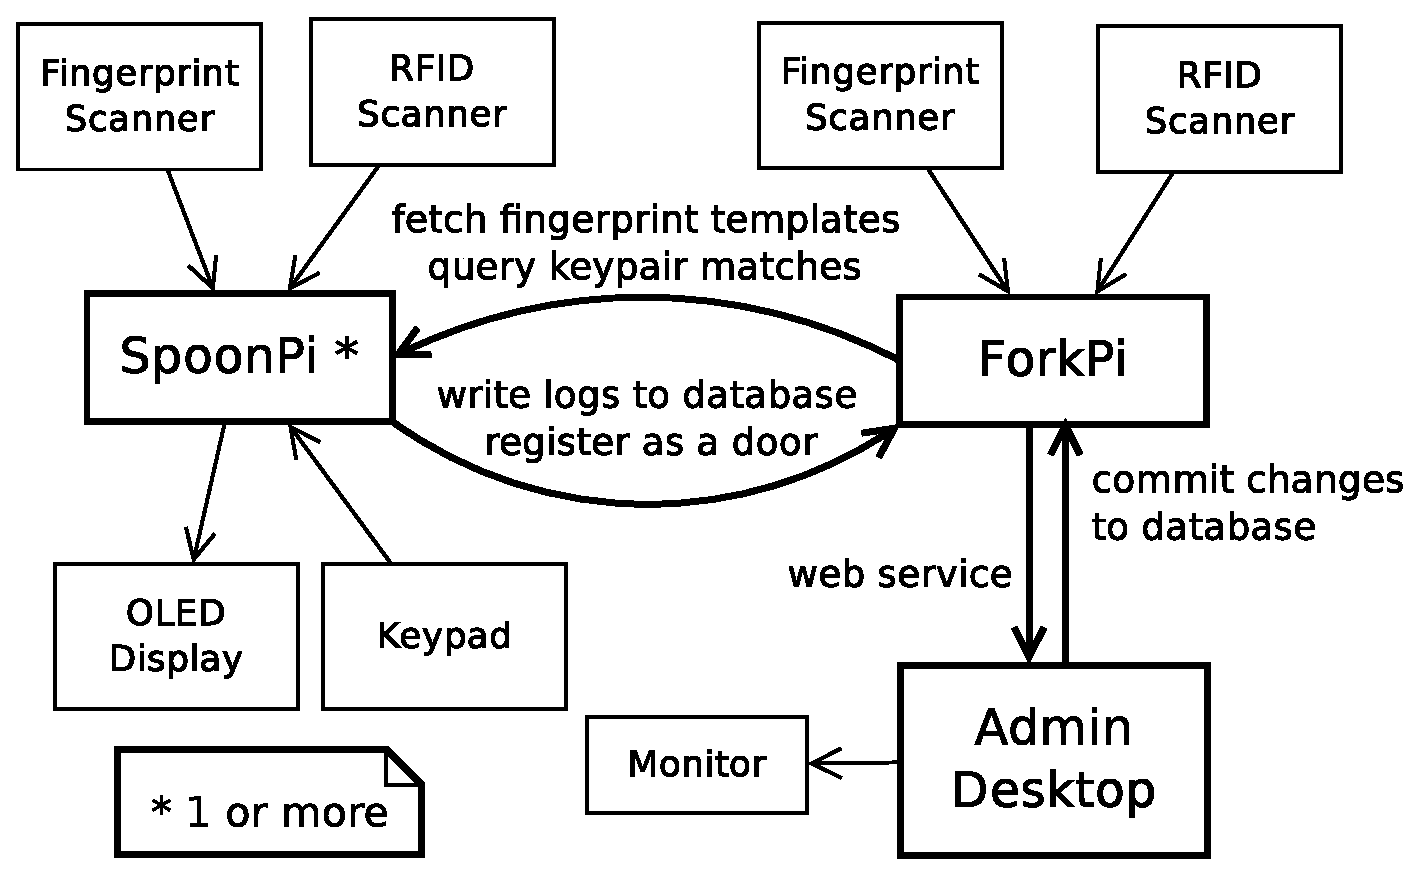
\includegraphics[scale=0.5]{architecture.eps}
\end{itemize}
\end{frame}

\subsection{ForkPi}
\begin{frame}{ForkPi Overview}
\begin{itemize}
    \item<1-> The ForkPi unit functions as both a web and database server.
    \item<2-> The web server runs a locally accessible website where one can register new users into the system, view logs, and perform other administrative actions.
    \item<3-> The web server has an underlying database run by PostgreSQL.
    \item<4-> Human administrators view ForkPi as a web server, while SpoonPis view ForkPi as a database server.
\end{itemize}
\end{frame}

\begin{frame}{Technical Overview}
\begin{itemize}
    \item<1-> ForkPi is addressed within the local network using the name forkpi.local, at HTTP port 80.
    \item<2-> The database server runs in the port 5432, so SpoonPis will access the database using the host name forkpi.local and the port number 5432.
    \item<3-> A dedicated ForkPi unit does not require the presence of a keypad nor an OLED display, but it requires having the following peripherals attached:
    \begin{itemize}
    	\item<4-> \textbf{RFID Scanner}: for scanning the UIDs of RFID tags to be registered
		\item<5-> \textbf{Fingerprint Scanner}: for the enrollment of new Fingerprints
    \end{itemize}
\end{itemize}
\end{frame}

\begin{frame}{Use Case Diagram}
\begin{itemize}
    \item<1-> 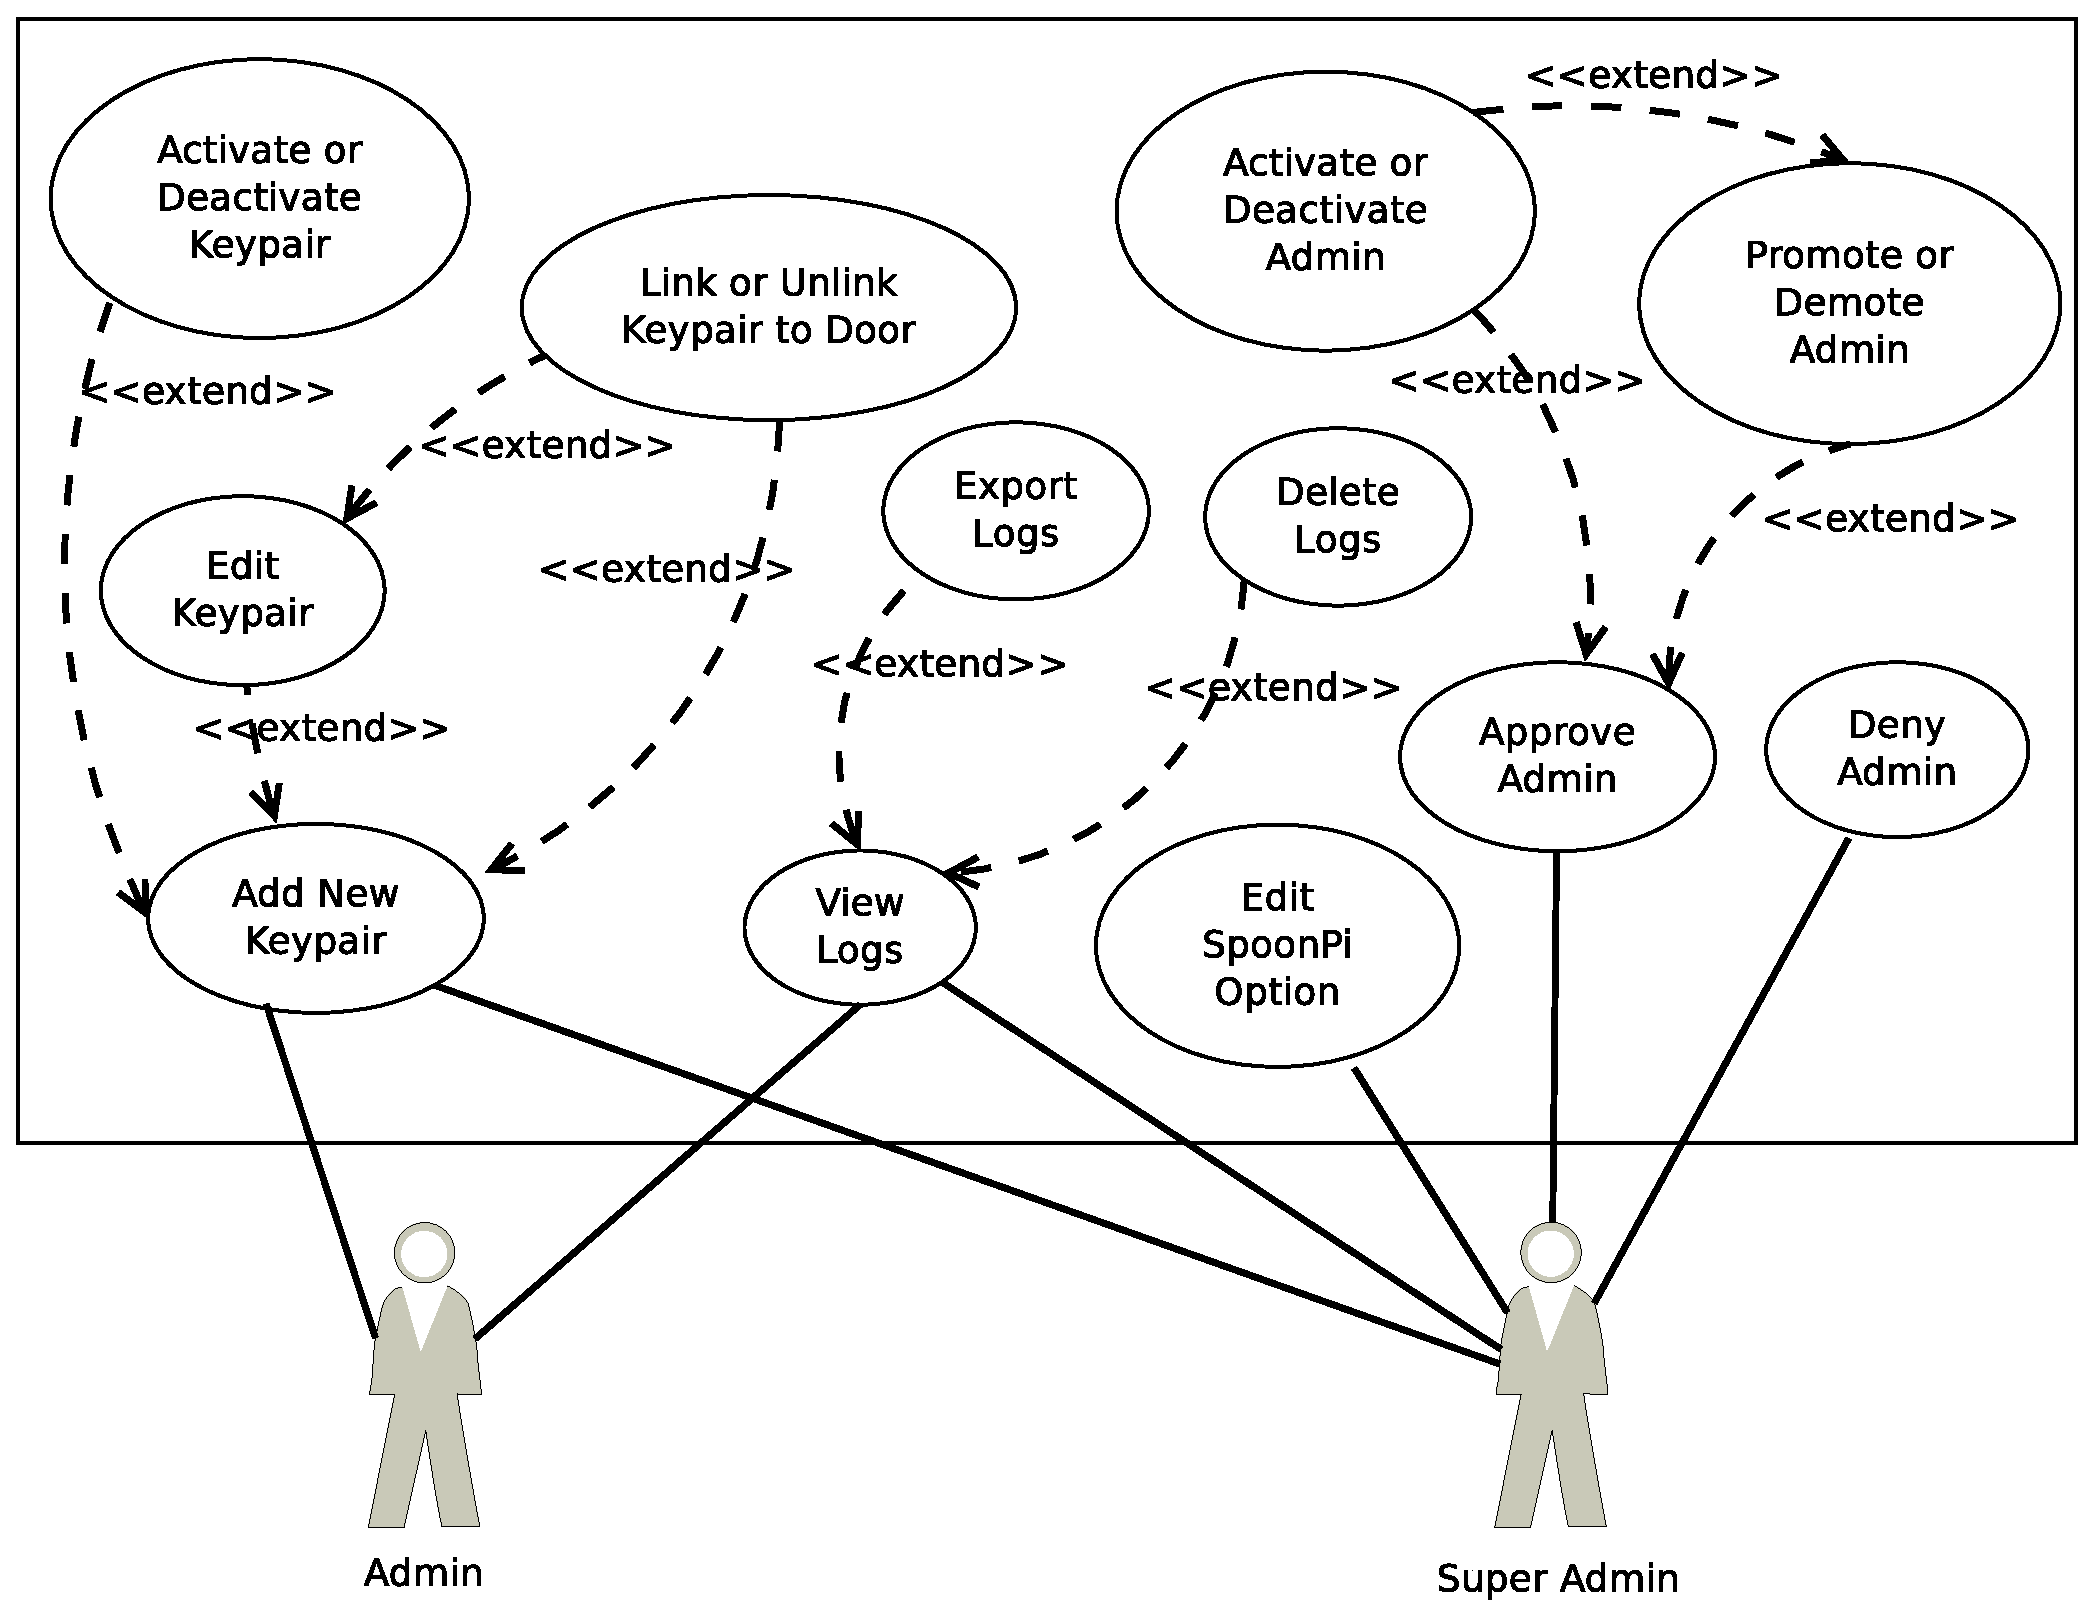
\includegraphics[scale=0.3]{forkpi-use-case.eps}
\end{itemize}
\end{frame}

\begin{frame}{Types of Admins}
\begin{itemize}
    \item<1-> There are two types of admins: regular admins and super admins.
    \item<2-> Super admins can perform everything a regular admin can do, with some additional functions we deemed to be potentially destructive in the hands of the wrong person. %% *SUCH AS???
    \item<3-> Regular admins have a limited set of permissions, and they can only become super admins with the consent of another super admin, in a process called promotion.
    \item<4-> New admin sign up requires the approval of another admin, and is a regular admin by default.
    \item<5-> However, if the system is new, admin sign up is automatically approved and is a super admin by default.
\end{itemize}
\end{frame}

\subsection{SpoonPi}
\begin{frame}{SpoonPi Overview}
\begin{itemize}
    \item<1-> The SpoonPi units serve as the media for door authentication, and are responsible for granting or denying access through doors. There are as many SpoonPis as doors to be secured.
    \item<2-> Each SpoonPi unit needs to register itself first with the ForkPi unit before any authentication can be done.
    \item<3-> SpoonPi performs authentication by communicating with the hardware components (e.g. RFID scanner) to get the input credentials (e.g. RFID UID), then querying the ForkPi database to check if it is valid.
    \item<4-> For fingerprint authentication, the verification is done at the SpoonPi side instead of the ForkPi side, because the matching is not a simple string comparison; fingerprint templates have to be uploaded to the scanner, where the actual matching takes place.
\end{itemize}
\end{frame}

\begin{frame}{Technical Overview}
\begin{itemize}
    \item<1-> A SpoonPi unit requires having the following peripherals attached:
    \begin{itemize}
    	\item<2-> \textbf{Fingerprint Scanner}: for identifying the fingerprint presented
		\item<3-> \textbf{OLED}: for displaying the current status of the transaction
		\item<4-> \textbf{RFID} Scanner: for scanning the UID of the RFID tag presented
		\item<5-> \textbf{Keypad}: for entering the PIN
    \end{itemize}
\end{itemize}
\end{frame}

\begin{frame}{SpoonPi Flowchart}
\begin{itemize}
    \item<1-> The following flowchart describing the main transaction loop:
    \item<2-> 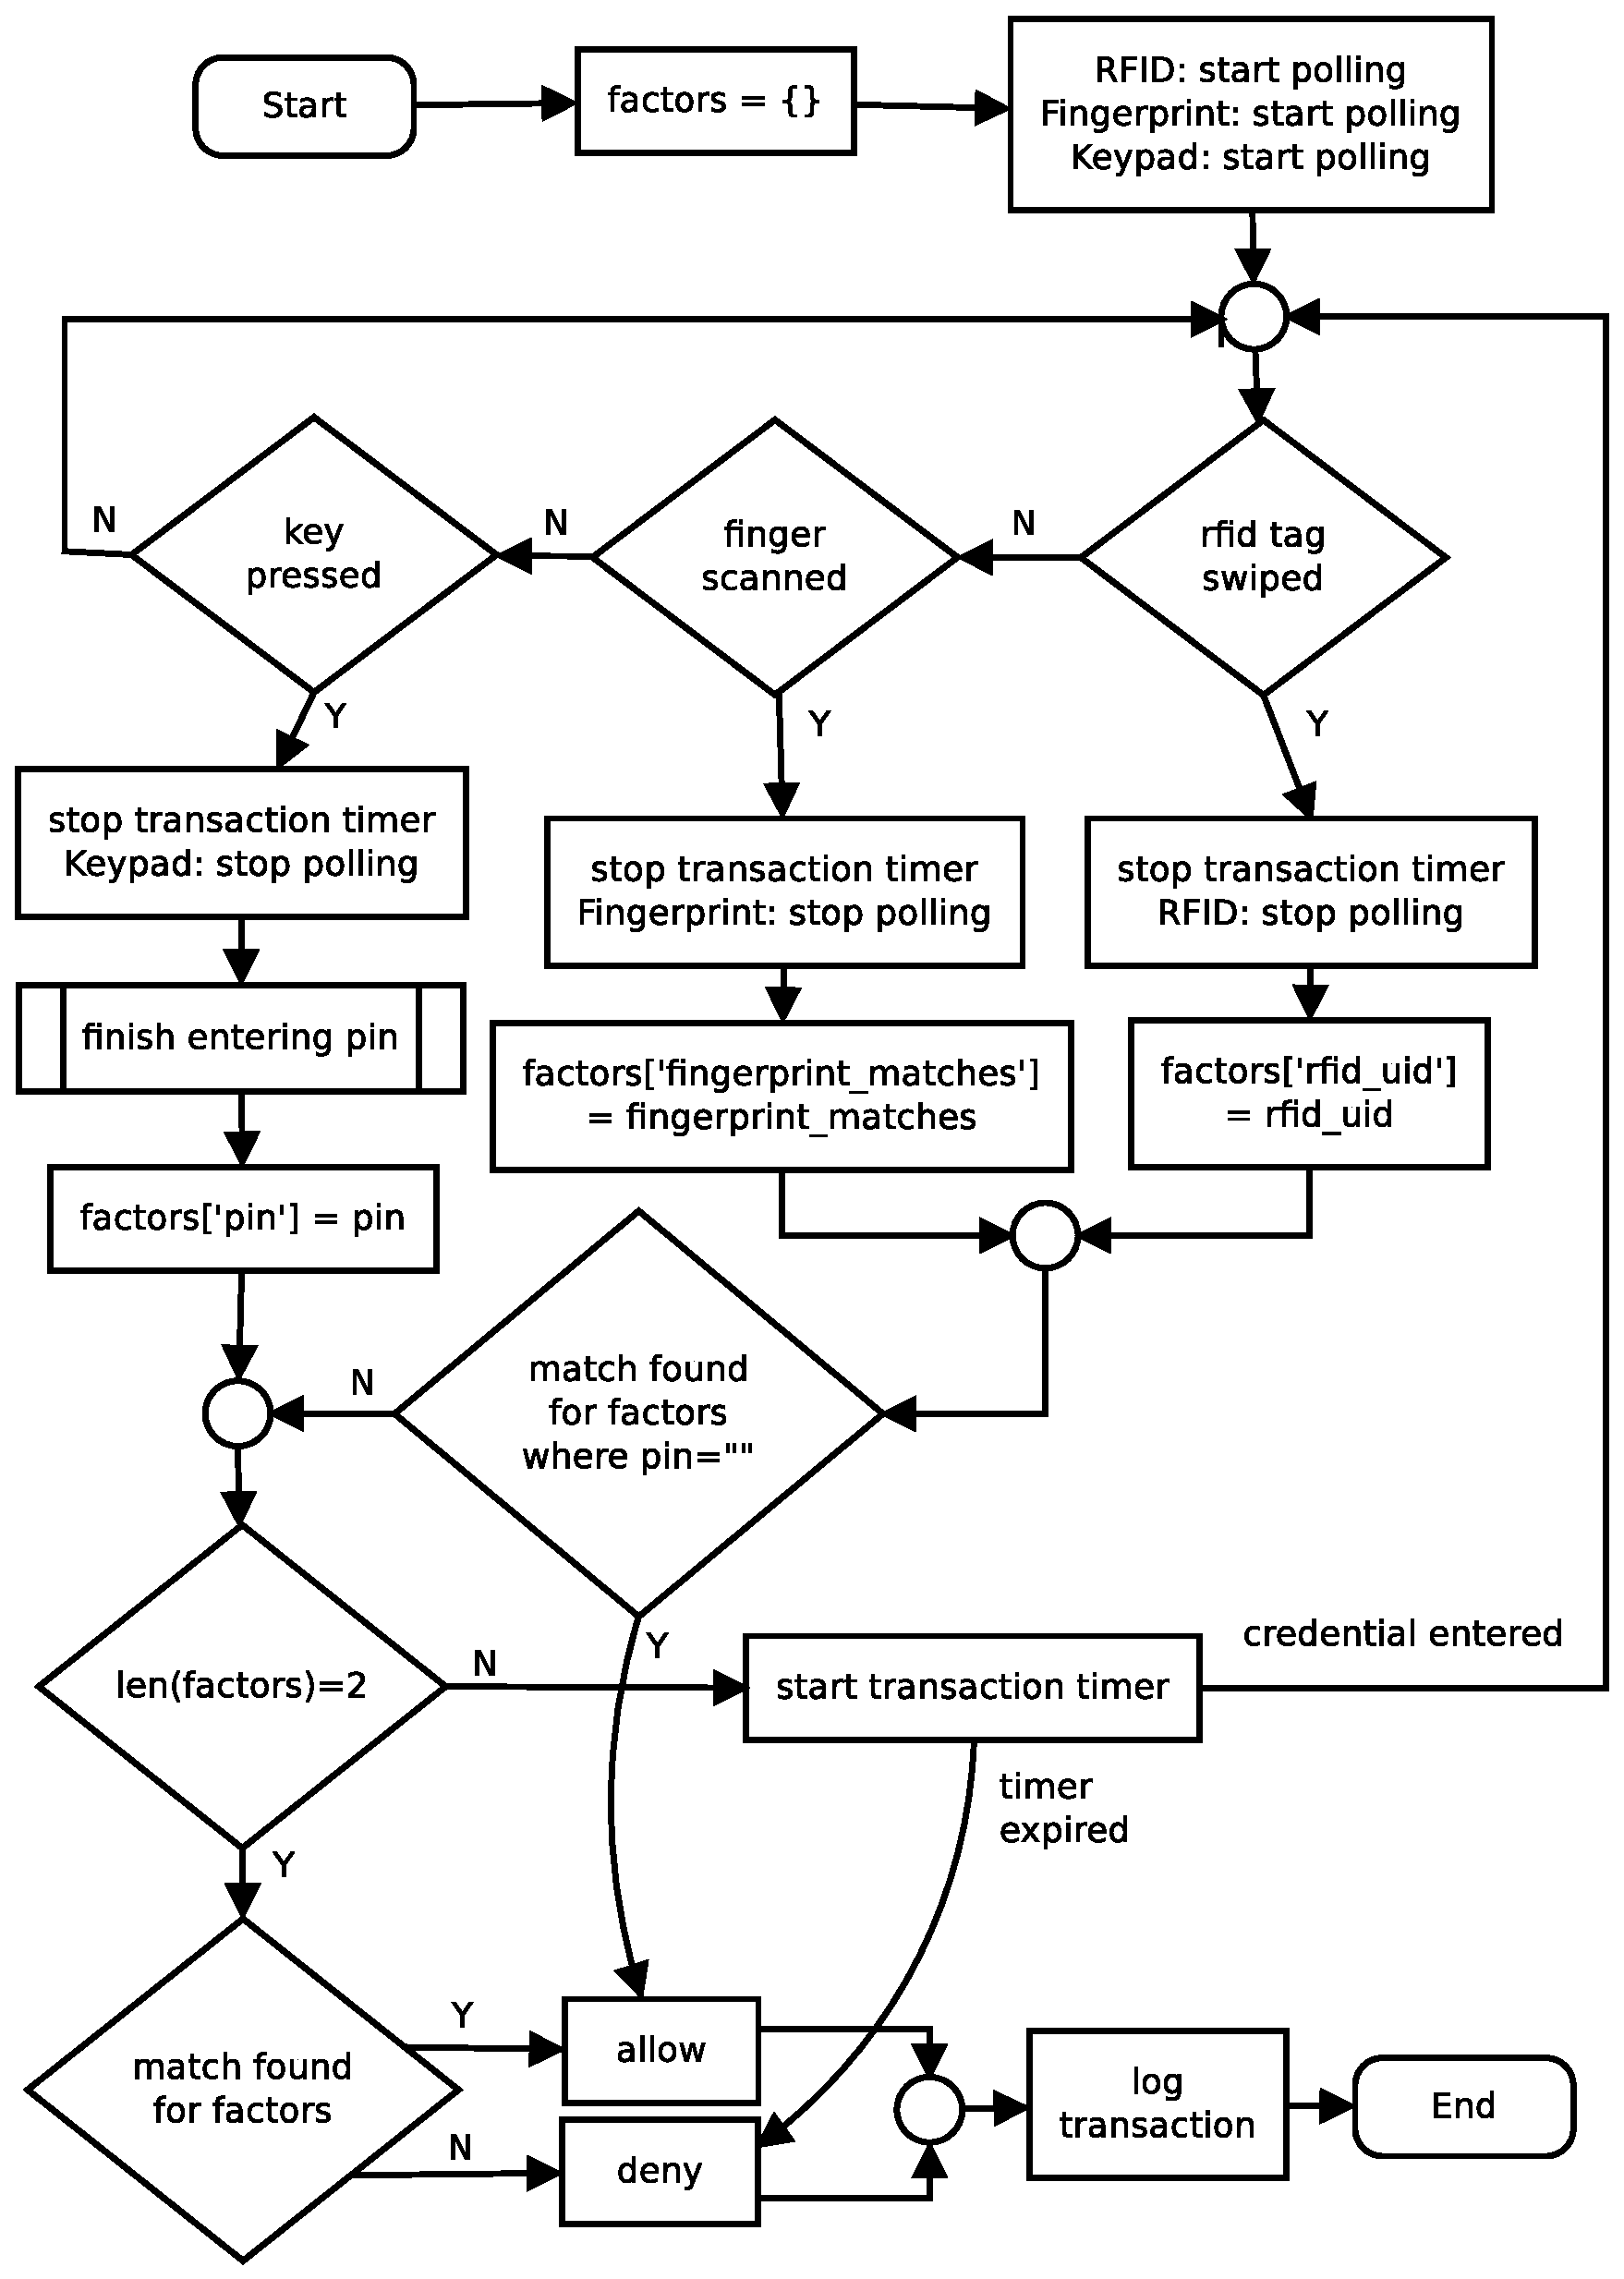
\includegraphics[scale=0.2]{spoonpi-flowchart.eps}
\end{itemize}
\end{frame}

\begin{frame}{SpoonPi PIN Flowchart}
\begin{itemize}
    \item<1-> The following flowchart describing the PIN input loop:
    \item<2-> 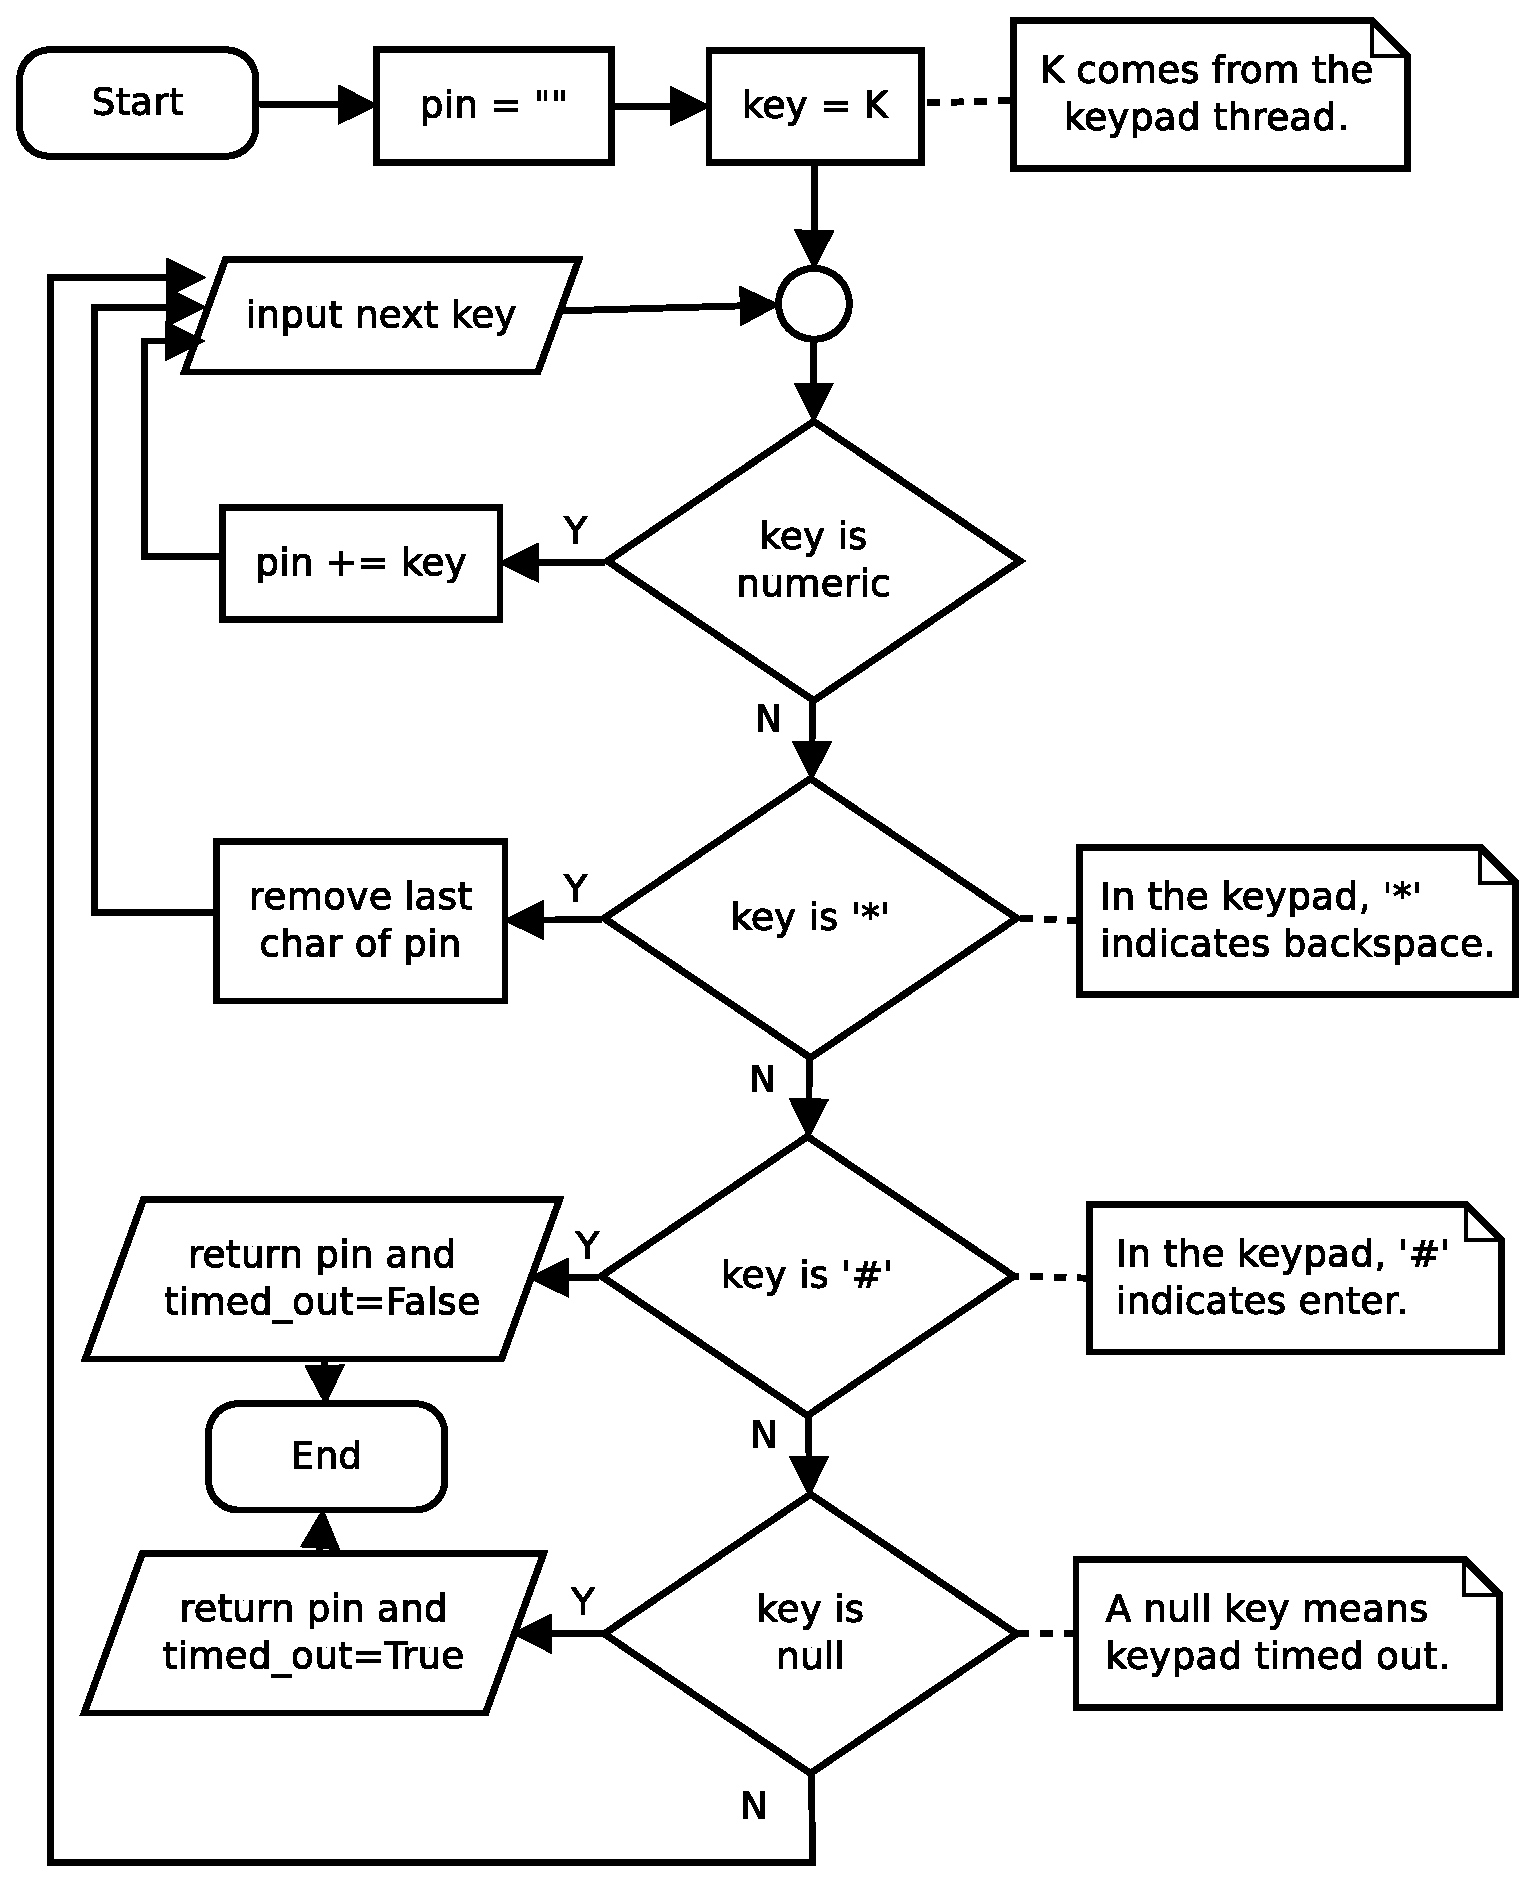
\includegraphics[scale=0.32]{pin-input.eps}
\end{itemize}
\end{frame}

\subsection{Security Options}
\begin{frame}{Security Options (1 of 2)}
\begin{itemize}
    \item<1-> \textbf{Attempt Limit}: The maximum streak of failed attempts where an RFID tag is presented and the wrong PIN is entered. This is to prevent guessing the PIN via brute force if an RFID tag is cloned or falls into an attacker's hands. The default value is 5 attempts.
    \item<2-> \textbf{Lockout Time (minutes)}: This is the amount of time to block the RFID tag from further use once the incorrect streak reaches the attempt limit. The default value is 30 minutes.
    \item<3-> \textbf{Keypad Timeout (seconds)} This is the maximum amount of time between key presses. The default value is 5 seconds.
\end{itemize}
\end{frame}

\subsection{Security Options}
\begin{frame}{Security Options (2 of 2)}
\begin{itemize}
    \item<1-> \textbf{Max Transaction Time (seconds)}: This is the maximum amount of time between presenting two authentication tokens. The default value is 10 seconds.
    \item<2-> \textbf{Lock Release Time (seconds)}: This is the amount of time to release the lock upon a successful attempt. The default value is 5 seconds.
\end{itemize}
\end{frame}

\section{Evaluation}
\subsection{Security}
\begin{frame}{Security of the PIN Component (1 of 3)}
\begin{itemize}
	\item<1-> Let's consider an attacker Oscar, who is trying to gain unauthorized access to a door by exploiting weaknesses inherent to a certain authentication factor used in the system.
    \item<2-> The main security concern with PIN is its vulnerability to brute force attacks.
    \item<3-> If an attacker Oscar gets hold of an authorized RFID tag, he can gain access to a door if he guesses the corresponding PIN.
    \item<4-> However, a lockout functionality has been implemented for RFID authentication, so Oscar has to wait a long time between guesses.
\end{itemize}
\end{frame}

\begin{frame}{Security of the PIN Component (2 of 3)}
\begin{itemize}
	\item<1-> The following formula is the average time it takes to guess a PIN using brute force in the system:
	$$T = (g \cdot t) + (L \cdot \frac gn) $$
	\item<2-> Where:
	\begin{itemize}
		\item<3-> $g$ is the average number of guesses needed
		\item<4-> $t$ is the average time it takes to try out a single PIN
		\item<5-> $L$ is the waiting time after a single lock-out
		\item<6-> and $n$ is the number of wrong attempts it takes before being locked-out.
	\end{itemize}
\end{itemize}
\end{frame}

\begin{frame}{Security of the PIN Component (3 of 3)}
\begin{itemize}
	\item<1-> On average, Oscar only needs to enter half of all possible PINs before guessing the correct one.
	\item<2-> There is no maximum PIN length imposed, which means the number of possible PINs is theoretically infinite, but assuming the following:
	\begin{itemize}
		\item<3-> All users use 6-digit PINs
		\item<4-> It takes 5 seconds to try out a single PIN.
		\item<5-> Lockout time is 30 minutes (default) 
		\item<6-> Attempt limit is 5 (default) 
	\end{itemize}
	\item<7-> Hence, $ g = \frac12 \cdot 10^6 = 500,000 \:\mathrm{guesses}, t = 5 \:\mathrm{s}, L = 1800 \:\mathrm{s}, n = \mathrm{5}$
	\item<8-> Plugging in those values, it would take, on average, $50694$ hours, or about $5.78$ years to crack. This makes brute force an impractical attack to use.
\end{itemize}
\end{frame}

\begin{frame}{Security of the RFID Component (1 of 2)}
\begin{itemize}
    \item<1-> The primary concern with RFID security is the issue of stolen or replicated tags.
    \item<2-> While we cannot prevent tags from being stolen, this is not a problem because our system allows admins to edit or deactivate keypairs.
    \item<3-> Hence, the user simply needs to go to the admin to get his keypair changed or deactivated.
\end{itemize}
\end{frame}

\begin{frame}{Security of the RFID Component (2 of 2)}
\begin{itemize}
    \item<1-> Replication of an RFID tag can be performed by scanning its UID, and reprogramming another tag to have the same UID.
    \item<2-> Attackers do not need to have access to the actual tag, as they can find out the UID simply by placing keyloggers near the RFID reader and waiting for it to be scanned.
    \item<3-> The MiFare cards we used cannot have their UIDs reprogrammed \footfullcite{MiFareAdafruit}, but some MiFare cards are made specially for cloning purposes (called ``magic'' MiFare cards).
    \item<4-> MiFare in general is not known to be secure, as some attacks have been developed for it. De Koning Gans et al recommend that a more advanced RFID card technology with an open design architecture be used over MiFare \footfullcite{de2008practical}.
\end{itemize}
\end{frame}

\begin{frame}{Security of the Fingerprint Component (1 of 2)}
\begin{itemize}
    \item<1-> The problem with fingerprint security is the possibility of generating false positives and false negatives. 
    \item<2-> While a false negative (denying a user that is supposed to be authorized) might cause some minor inconvenience on the part of the user, a false positive (allowing a user that is not supposed to be authorized) is potentially devastating.
    \item<3-> However, an attacker cannot rely solely on chance in order to generate a false positive, since that probability is infinitesimally small (less than 0.00001\% in our case).
\end{itemize}
\end{frame}

\begin{frame}{Security of the Fingerprint Component (2 of 2)}
\begin{itemize}
    \item<1-> What the attacker can do is to make a clone of the registered fingerprint. This can be done by pressing the finger against various materials such as silicone or gelatin, in order to make a mold.
    \item<2->  We have not personally tested our fingerprint scanner against such clones, but in the study done by Matsumoto et al on 11 fingerprint scanners, they found that 67\% of them accepted the gummy fingers \footfullcite{matsumoto2002impact}.
    \item<3-> Hence, it is not unreasonable to assume that our scanner will also be deceived by artificial fingers.
    \item<4-> However, this attack relies on the attacker obtaining an accurate mold of the finger, which usually requires the cooperation and consent of the authorized user.
\end{itemize}
\end{frame}

\begin{frame}{Security Against Passive Attacks (1 of 2)}
\begin{itemize}
    \item<1-> Let us assume that an eavesdropper Eve can read all messages being passed between SpoonPi and ForkPi, and ForkPi and the admin’s computer.
    \item<2-> While Eve can listen in on the exchanges, she cannot modify them.
    \item<3-> Hence, our system is secure against such attacks for both communication lines.
    \item<4-> \textbf{Communication between SpoonPi and ForkPi}: When a PIN is entered or an RFID UID is scanned, SpoonPi never queries for matches in plaintext. These two fields are hashed first using SHA-1, so Eve cannot retrieve their original values.
\end{itemize}
\end{frame}

\begin{frame}{Security Against Passive Attacks (2 of 2)}
\begin{itemize}
    \item<1-> \textbf{Communication between ForkPi and the admin’s computer}:
    \begin{itemize}
    	\item<2-> In the web application, it becomes more difficult to safely transmit the PIN and RFID UID without exposing them to Eve, since admins need to be able to view them in plaintext.
    	\item<3-> When an admin logs in, the authentication credentials are not included in the web page. However, when the admin edits a user’s keypair, his/her credentials will be sent to ForkPi in plaintext.
    	\item<4-> The same goes for when the admin adds a new keypair; the new keypair’s credentials might be exposed to Eve. The impact is lessened in a system with multiple doors, since it would become more difficult for Eve to determine which door(s) a keypair is linked to.
    \end{itemize}
\end{itemize}
\end{frame}

\begin{frame}{Security Against Active Attacks (1 of 3)}
\begin{itemize}
    \item<1-> Let us assume that a malicious attacker, Mallory, is actively trying to break into the security of the system, either by targeting a single computer, or by pretending to be a certain computer to another computer.
\end{itemize}
\end{frame}

\begin{frame}{Security Against Active Attacks (2 of 3)}
\begin{itemize}
    \item<1-> \textbf{Attack on the Database}:
    \begin{itemize}
    	\item<2-> If Mallory was able to guess the username and password of the PostgreSQL database, she would gain access to it.
    	\item<3-> However, she will not be able to retrieve the PIN and RFID UID in plaintext, since they are encrypted in 128-bit AES.
    	\item<4-> Gaining access to the database can still potentially damage the system because Mallory can delete all the tables and rows. This is a severe attack on the system, so it is highly recommended to have a strong username and password for PostgreSQL.
    \end{itemize}
\end{itemize}
\end{frame}

\begin{frame}{Security Against Active Attacks (3 of 3)}
\begin{itemize}
    \item<1-> \textbf{Man In The Middle Attack}:
    \begin{itemize}
    	\item<2-> All computers in the local network refer to ForkPi using \texttt{forkpi.local}
    	\item<3-> Theoretically, Mallory can create a naming collision with ForkPi by setting her own computer’s hostname to forkpi, and then running a service under the name \texttt{forkpi.local}.
    	\item<4-> However, the service discovery software that we use, Avahi, resolves name collisions by appending a number to the hostname (e.g. \texttt{forkpi-2.local}), in accordance with the Zeroconf protocol \footfullcite{rfc6762}.
    	\item<5-> These numbers are assigned according to the order of start-up. Hence, provided that the ForkPi unit is started before Mallory's computer, \texttt{forkpi.local} will refer to the real ForkPi unit. Therefore, it will be hard for Mallory to pass off her own computer as the ForkPi unit.
    \end{itemize}
\end{itemize}
\end{frame}

\subsection{Usability}
\begin{frame}{Usability (1 of 4)}
\begin{itemize}
    \item<1-> The following figure shows the list of questions and the amount of respondents for each possible response.
    \item<2-> 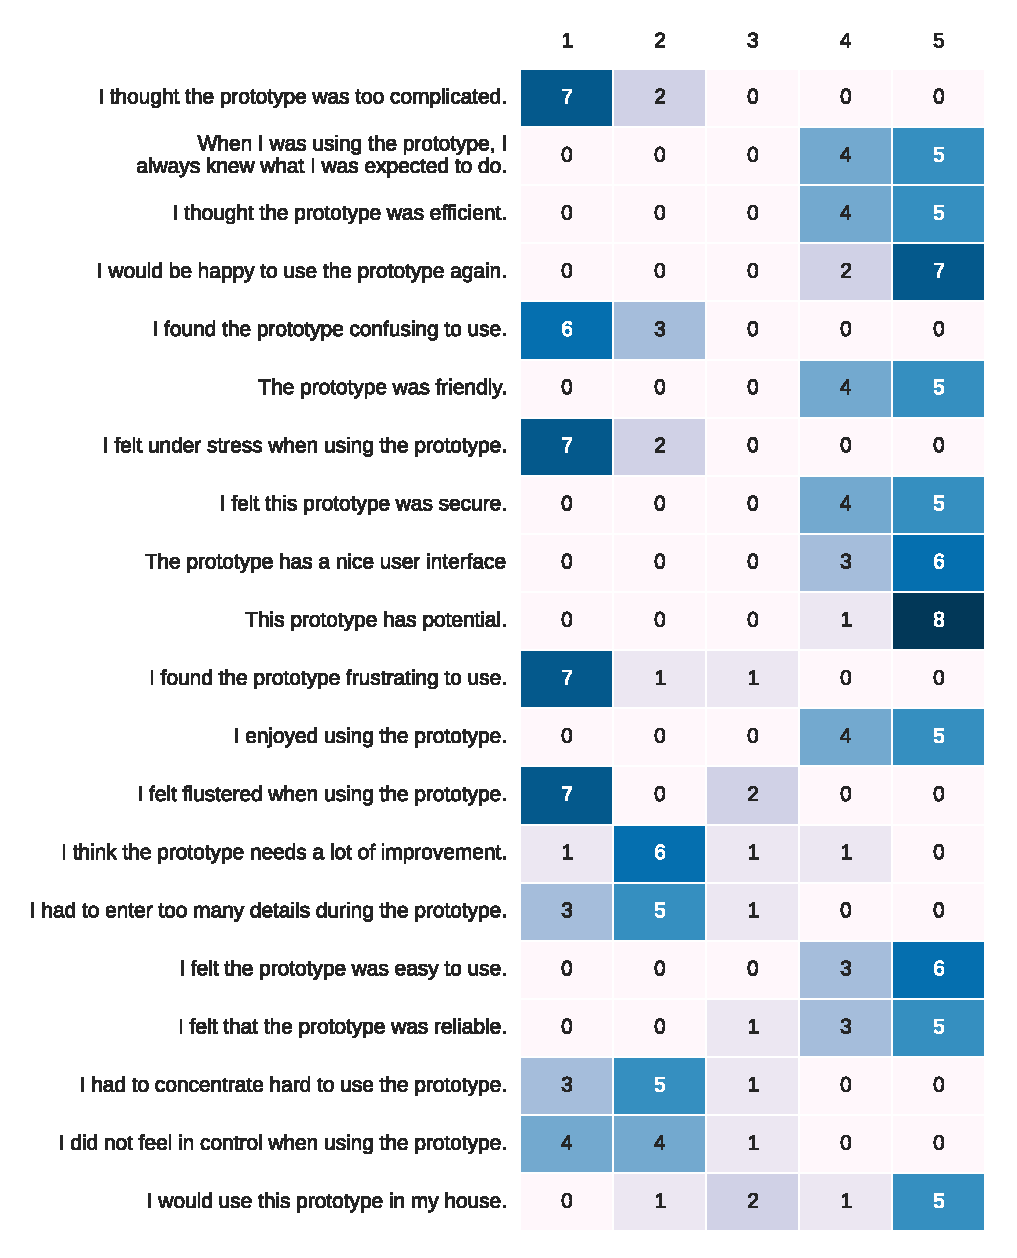
\includegraphics[scale=0.25]{uat-results.eps}
\end{itemize}
\end{frame}
\begin{frame}{Usability (2 of 4)}
\begin{itemize}
    \item<1-> Some of the questions were phrased negatively in order to ensure that the respondents are reading the questions carefully.
    \item<2-> There was a total of nine respondents from different walks of life:
    \begin{itemize}
        \item<3-> Four of the respondents were female, while five were male.
        \item<4-> Four of the respondents were within the 18 to 25 age range, the other four were within the 26 to 40 age range, and the remaining respondent was aged 68.
    \end{itemize}
\end{itemize}
\end{frame}

\begin{frame}{Usability 3 of 4)}
\begin{itemize}
    \item<1-> The following figure shows the list of respondents and their answers, grouped by their answer to the question, ``Have you ever operated/used a door access control system before?''
    \item<2-> 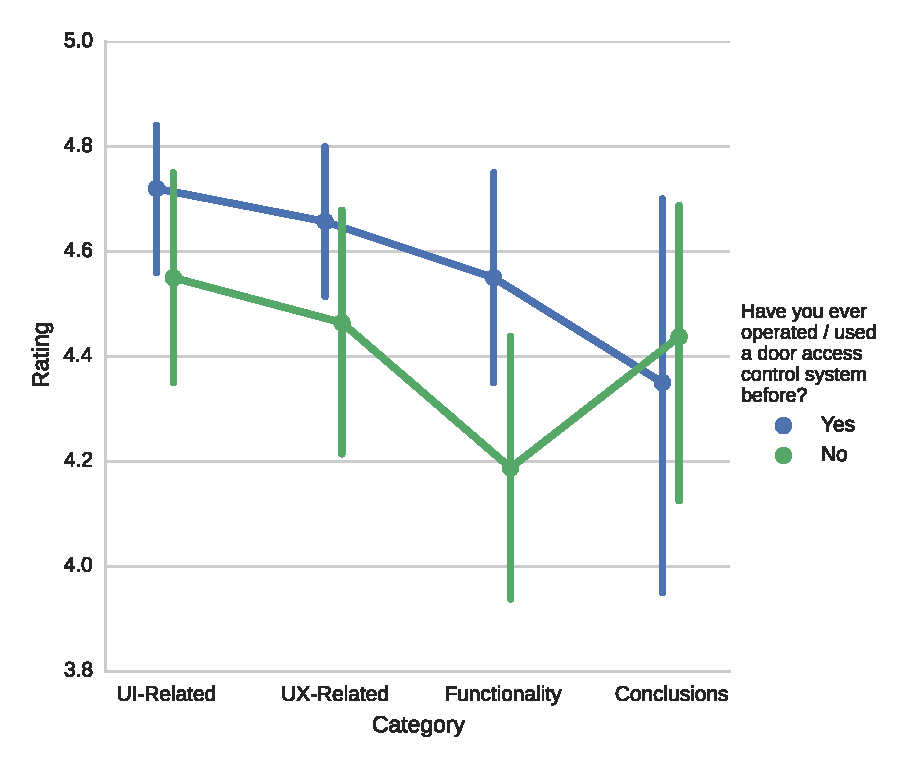
\includegraphics[scale=0.7]{tech-non-tech.eps}
\end{itemize}
\end{frame}

\begin{frame}{Usability 4 of 4)}
\begin{itemize}
    \item<1-> Five of the respondents had no experience at all with keyless door access control systems.
    \item<2-> The respondents who had no experience reviewed the system less favorably, as opposed to the respondents who had experience.
    \item<3-> An exception, however, occurs with questions pertaining to drawing conclusions from the system (e.g. ``The prototype has potential.''), where the respondents with no experience ranked the system more favorably.
    \item<4-> Overall, the respondents rated the system positively, commenting that the system shows promise and has a lot of potential, especially compared to products that are currently in the market.
\end{itemize}
\end{frame}

\subsection{Cost-Effectiveness}
\begin{frame}{Cost-Effectiveness (1 of 3)}
\begin{itemize}

    \item<1-> In this section, we list all the hardware components we used for the system, along with their respective prices.
    \item<2-> We then compare the prices of each component against the prices of similar components that can be purchased from the online store Amazon \footfullcite{Amazon}.
    \item<3-> We also compare the total price of our system against similar commercial products that are for sale on Amazon.
    
\end{itemize}
\end{frame}

\begin{frame}{Cost-Effectiveness (2 of 3)}
\begin{itemize}

    \item<1-> In determining the price ranges, we took a look at the price filters on Amazon, and for each price range, we multiplied the number of items by the maximum amount in that range. (e.g.: For the \$200 and above price, we set the price to \$250.)
    \item<2-> In determining the lower end of the range, we set the count of the most expensive group to 0, and took the mean price. For the higher end, we set the count of the least expensive group to 0, and took the mean price.
    
\end{itemize}
\end{frame}

\begin{frame}{Cost-Effectiveness}
\begin{table}[h]
	\centering
	\begin{threeparttable}
	\begin{tabular}{lll|l|l|}
	\cline{4-5}
	 &  &  & \multicolumn{2}{c|}{Cost} \\ \hline
	\multicolumn{1}{|l|}{} & \scriptsize{Component} & & \scriptsize{Project} & \scriptsize{Commercial} \\ \hline
	\multicolumn{1}{|l|}{Base} & \scriptsize{Raspberry Pi Model B} &  & \scriptsize{\$35} & \scriptsize{\$35} \\
	\multicolumn{1}{|l|}{} & \scriptsize{OLED Display} &  & \scriptsize{\$17.50} & \scriptsize{\$10 - \$20} \\
	\multicolumn{1}{|l|}{} & \scriptsize{Raspberry Pi Cobbler Breakout} &  & \scriptsize{\$6.50} & \scriptsize{\$6 - \$11} \\ \hline
	\multicolumn{1}{|l|}{PIN} & \scriptsize{Keypad} &  & \scriptsize{\$3.95} & \scriptsize{\$2.5 - \$7} \\ \hline
	\multicolumn{1}{|l|}{RFID} & \scriptsize{Reader} &  & \scriptsize{\$39.95} & \scriptsize{\$30 - \$80} \\
	\multicolumn{1}{|l|}{} & \scriptsize{MiFare Classic 13.56MHz Card x1} &  & \scriptsize{\$2.50} & \scriptsize{\$0.5 - \$1.5} \\
	\multicolumn{1}{|l|}{} & \multicolumn{2}{r|}{\scriptsize{Total (Base+RFID+PIN)}} & \scriptsize{\$102.9} & \scriptsize{\$80 - \$140} \\ \hline
	\multicolumn{1}{|l|}{Fingerprint} & \scriptsize{Scanner} &  & \scriptsize{\$49.95} & \scriptsize{\$40 - \$90} \\
	\multicolumn{1}{|l|}{} & \multicolumn{2}{r|}{\scriptsize{Total (Base+Fingerprint+PIN)}} & \scriptsize{\$110.4} & \scriptsize{\$100 - \$170} \\ \hline
	\multicolumn{1}{|l|}{} & \multicolumn{2}{r|}{\scriptsize{Total (All Components)}} & \scriptsize{\$152.85} & \scriptsize{\$140 - \$200} \\ \hline
	\end{tabular}
	\end{threeparttable}
	\end{table}

\end{frame}
\section{Recommendations}
\subsection{Recommendations}
\begin{frame}{Recommendations}
\begin{itemize}
    \item<1-> In this section, we discuss some of the limitations of our system, and propose various improvements to it.
    \item<2-> These improvements can be implemented by future researchers who plan to either continue this project, or create similar door access control systems.
    \item<3-> Improvements are classified into two categories:
    \begin{itemize}
    	\item<4-> Vital to use the system in a real world setting
    	\item<5-> Potentially useful as extra features.
	\end{itemize}
\end{itemize}
\end{frame}

\subsection{Core Functionality}
\begin{frame}{Communication with Door Lock}
\begin{itemize}
    \item<1-> When implementing the system, a door lock module needs to be installed in the Raspberry Pi.
    \item<2-> In the code, however, we have created a dummy door lock class which we give instructions to, like \texttt{lock} or \texttt{unlock}, so that future researchers will have less trouble implementing the real door lock class.
\end{itemize}
\end{frame}

\begin{frame}{Exit Button}
\begin{itemize}
    \item<1-> Since the SpoonPi controller is only installed outside the room, users who are inside the room need a way to mechanically disable the lock in order to leave the room.
    \item<2-> An exit button needs to be connected to the door lock, in order to temporarily unlock it when it is pressed.
    \item<3-> This can be implemented using pure hardware wiring; it does not necessarily have to pass through the SpoonPi unit.
\end{itemize}
\end{frame}

\begin{frame}{Power Supply}
\begin{itemize}
    \item<1-> In real world systems, we cannot assume that the power will be consistently on.
    \item<2-> Before a SpoonPi unit loses power, it must be able to unlock all doors, or else someone might get locked inside a room.
    \item<3-> To solve this problem, the SpoonPi must be connected to an emergency power supply, and know how much battery life is left.
    \item<4-> Such a power supply would enable SpoonPi to function even after a power outage, and determine when to release all door locks and shut down.
    \item<5-> Another potential improvement for the system is the use of Power Over Ethernet (PoE), so that only one cord needs to be attached to each Raspberry Pi unit. With this, we can provide power and transmit data over the same wire.
\end{itemize}
\end{frame}

\begin{frame}{Connectivity Indicator}
\begin{itemize}
    \item<1-> Like the power supply, we cannot assume that all SpoonPi units will always be able to connect to the ForkPi database.
    \item<2-> If network connectivity fails, then SpoonPi will not be able to query ForkPi for keypair matches, hence the whole system falls apart.
    \item<3-> If we cannot recover from a network failure, we should at least be able to release control of the lock, and communicate the disconnectivity to users.
    \item<4-> This can be done in the form of a LED light that is only on when it is connected to ForkPi.
\end{itemize}
\end{frame}

\subsection{Useful Improvements}
\begin{frame}{Cached Keypairs}
\begin{itemize}
    \item<1-> Should SpoonPi lose its connectivity with ForkPi, SpoonPi has no way of determining which keypairs are authorized, so it has to release the door lock.
    \item<2-> Instead of querying the ForkPi database for every transaction, it would be better for the SpoonPi to maintain its own copy of authorized keypairs, so that it can function after a network failure.
    \item<3-> This can be implemented as a cached database copy, which is periodically updated whenever SpoonPi is connected to ForkPi.
\end{itemize}
\end{frame}

\begin{frame}{ForkPi Hierarchy}
\begin{itemize}
    \item<1-> In our system, there is only one ForkPi unit in the entire network. This makes ForkPi a single point of failure. % (why?)
    \item<2-> It is possible to introduce a hierarchy of ForkPis, such that there is a Raspberry Pi unit (called KnifePi) that is dedicated to talking to ForkPis, while the ForkPis are the ones that talk to the SpoonPis.
    \item<3-> Each ForkPi must be able to stand on its own without the help of KnifePi, so that KnifePi does not become a single point of failure.
    \item<4-> ForkPi units can be connected to different networks, as long as KnifePi can reach all of them. For example, one ForkPi can be dedicated to each floor, and one KnifePi for the entire building.
\end{itemize}
\end{frame}

\begin{frame}{Data Backup and Restore}
\begin{itemize}
    \item<1-> Since the memory on the ForkPi's SD card is limited, we want to be able to permanently delete obsolete data in order to free up space.
    \item<2-> In the ForkPi web app, we already provided a way to export logs to CSV, and delete them from the database.
    \item<3-> However, there is no easy way to back-up keypairs to a file such that they can be restored later if the need arises. 
    \item<4-> Theoretically, this can be done by dumping the PostgreSQL database and restoring it, but we want to be able to do this inside the web app for convenience.
\end{itemize}
\end{frame}

\begin{frame}{Date and Time-based Permissions}
\begin{itemize}
    \item<1-> In some environments, users can be granted access through a door only at a certain time of the day, or on certain days of the week.
    \item<2-> When a keypair is linked to a door, it might be beneficial to be able to specify at which specific times the keypair is valid for that door.
    \item<3-> For example, students should only be allowed into classrooms when they have a class at that time.
\end{itemize}
\end{frame}

\begin{frame}{Realtime Log Analysis}
\begin{itemize}
    \item<1-> Our logging system allows admins to review the logs and check for intruders in the system. In a system with thousands of users, manually checking the logs will become infeasible.
    \item<2-> Ideally, intrusion detection should be automatically done. For example, if the same keypair was presented to two SpoonPis at around the same time, then one of them might have been an intruder, especially of the two SpoonPis are geographically far apart.
    \item<3-> The hardware components, like the Pi controller or the door knob, can also be checked for damage, since an intruder may try physically breaking the system in order to get in by force.
\end{itemize}
\end{frame}

\subsection{Conclusion}
\begin{frame}{Conclusion(1 of 2)}
\begin{itemize}
    \item<1-> Our system aims to provide cost-effective security to the public.
    \item<2-> Since all the system components can be easily bought from online stores, and we made the code open source, any user that wants to try out the system can build the system for themselves.
    \item<3-> While the door lock has not yet been integrated into the system, all other major functions are already in place, like determining whether to allow a user based on their input credentials, managing user permissions, and viewing and exporting logs.
\end{itemize}
\end{frame}

\begin{frame}{Conclusion(2 of 2)}
\begin{itemize}
    \item<1-> Communications are encrypted, and additional features such as lockouts are implemented in order to defend against attackers.
    \item<2-> When we presented the system, it was well-received, whether the person had prior experience with similar systems or not.
    \item<3-> We have shown that the system is both acceptably secure, and easy to understand and operate, while still costing less than most commercial products currently available in the market.
\end{itemize}
\end{frame}

\end{document}